\documentclass[12pt]{article}
%\documentclass[12pt, letterpaper, twoside]{article}
\usepackage{graphicx}
\usepackage{xcolor}
\usepackage{subcaption}
\usepackage{hyperref}
\definecolor{linkcolour}{rgb}{0,0,1}
\hypersetup{colorlinks=true, urlcolor=linkcolour, linkcolor=linkcolour, linkbordercolor=linkcolour, pdfborderstyle={/S/U/W 1}} 
\urlstyle{same}

\usepackage{setspace} 
\singlespacing

\usepackage{geometry}
\geometry{margin=1in}

\setlength\parindent{0pt}

\graphicspath{{images/}}

\begin{document}
\title{Bike-Share Case Study}
\date{}
\maketitle

This report provides the results as well as the step-by-step explanation of the data analysis performed for a bike sharing case-study. The data belongs to a bike-sharing company that has two kinds of users: annual members and casual riders. The goal of the case-study was to identify how annual members and casual riders use the bikes differently in order to help the stake-holders decide whether or not to target converting casual riders into annual members in the next marketing campaign. The data used in this case-study was between January-November 2023, each month was stored in a csv file, and was downloaded from \url{https://divvy-tripdata.s3.amazonaws.com/index.html}. 

\section*{Data-Set exploration \& cleaning:}
The code that was used to perform the data exploration can be found in the Jupyter Notebook \href{https://github.com/SummerKassem/BikeShareCS/blob/main/Code/cleaning.ipynb}{cleaning.ipynb}. Below are the main functions:
\begin{itemize}
	\item \textit{read\_data}:\\
	Here the csv file for the bike rides of each month is read and stored into a dictionary called “data”. Each element in the dictionary has a key (the name of the month) and a value (the panada dataframe that holds the csv entries). This simplifies the access of the entries for each corresponding month, by using the month as the key (e.g. data[“February”] retrieves the dataframe that holds the entries from February). Below we can see the first and last 5 entries of bike rides from May (a couple of NaN values already show up).

	\begin{figure}[h]
	\hspace{-1.8cm}
	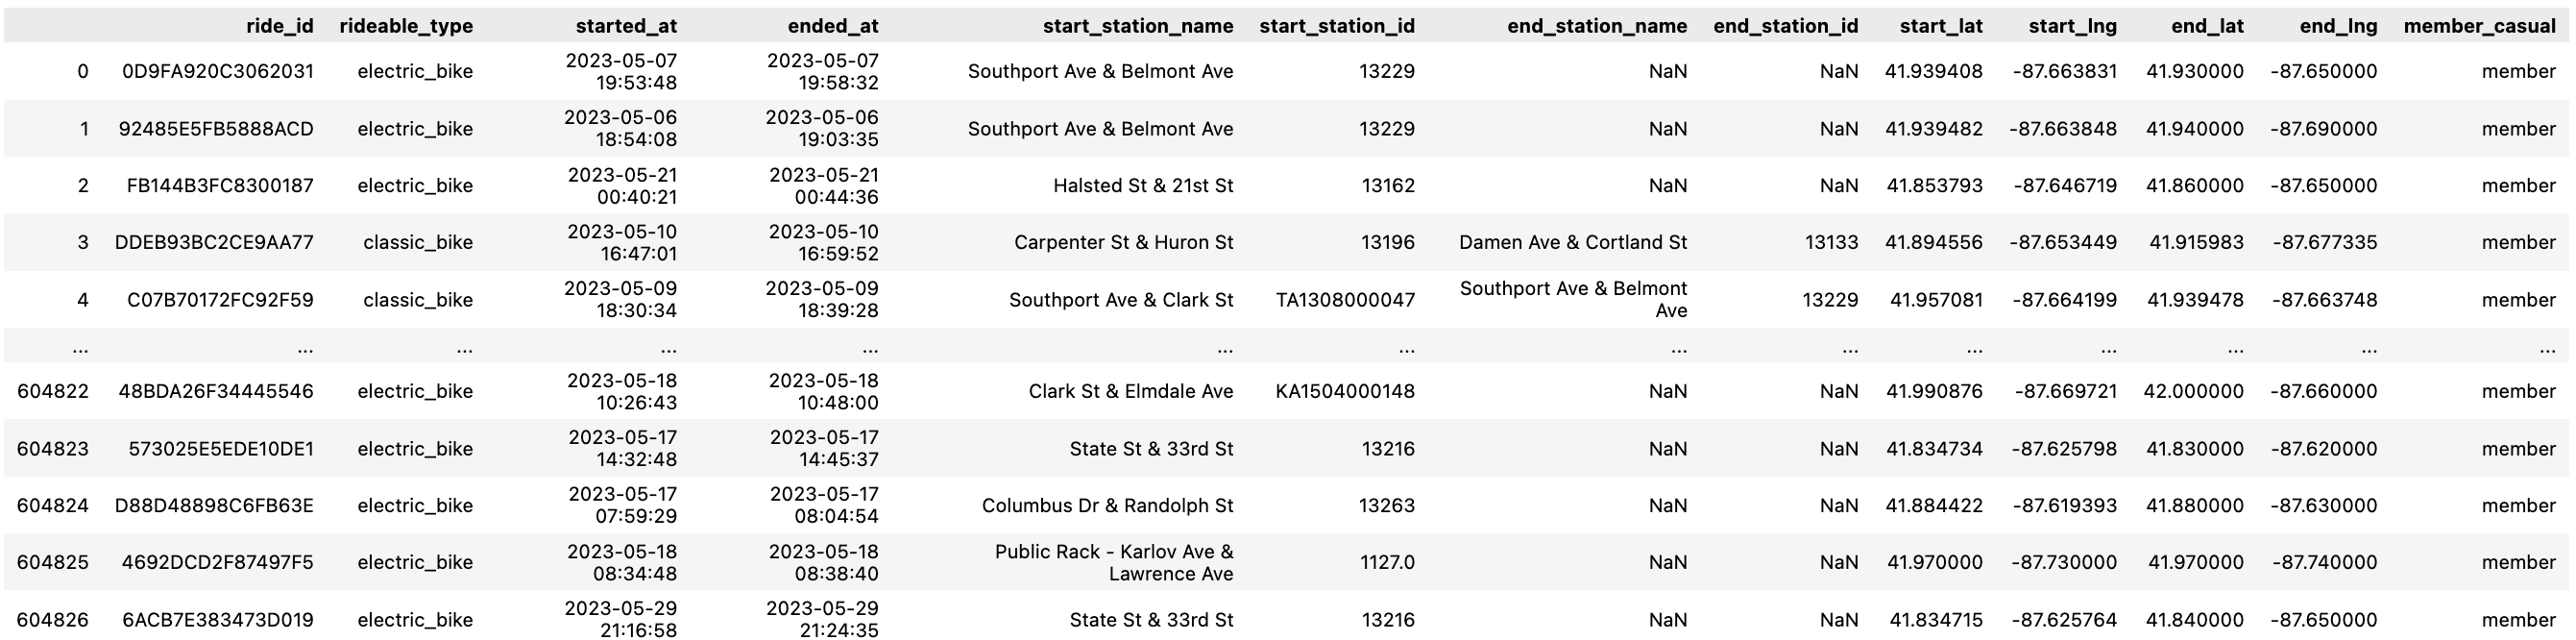
\includegraphics[width=8 in, height = 2 in]{imgMay.png}
	\end{figure}
	\pagebreak
	
	From the entries of data[``May"], we can see that the data for May consists of 13 columns: a ride id, the type of bike, date and time for the start and end of the ride, the name, id, latitude and longitude of the start and end stations, and finally whether the user was a casual rider or a member. In order to explore the dataset a bit further, the method \textit{nunique()} is used to return the number of unique values for each column. The output is shown below. 
	
	\begin{figure}[h]
	\centering
	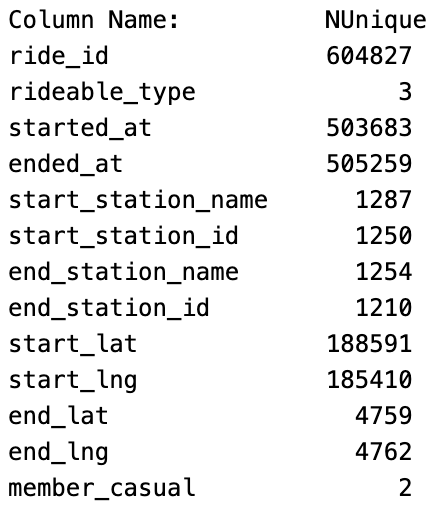
\includegraphics[scale = 0.6]{imgUnique.png} %[width=8 in, height = 2 in]
	\end{figure}
	
	Looking at the number of unique values, it seems that only the columns \textit{rideable\_type} and \textit{member\_casual} have unique values. The method \textit{unique()} is then be used to find these values:  
	\begin{itemize}
	\item \textit{rideable\_type}: [electric\_bike, classic\_bike, docked\_bike]
	\item	  \textit{member\_casual}: [member, casual]
	\end{itemize}
	
	\item \textit{count\_entries}:\\
	This method collects further information about the dataset. It finds the number of entries per file as well as the number of columns. This is done in order to validate the consistency of data across the different files. From these values the method then calculates the total number of bike rides in the entire dataset. There is an option within the method to remove duplicates. Therefore, the method is first called with the remove duplicates option deactivated, in order to get a preliminary feel of the dataset, how big it is, how the entires varies across the months. And then the method is called again with the remove duplicates option activated. The results are then written to output files which are shown below. 
	
	\begin{figure}[h]
	\centering
	\begin{subfigure}{.4\textwidth}
	\hspace{0.5 in}
		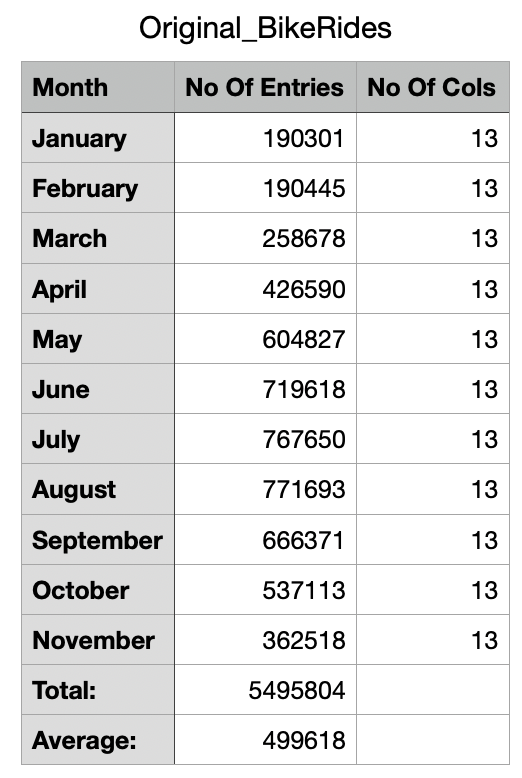
\includegraphics[scale=0.5]{img2.png}
	\end{subfigure}
	\begin{subfigure}{.4\textwidth}
	\hspace{0.5 in}
		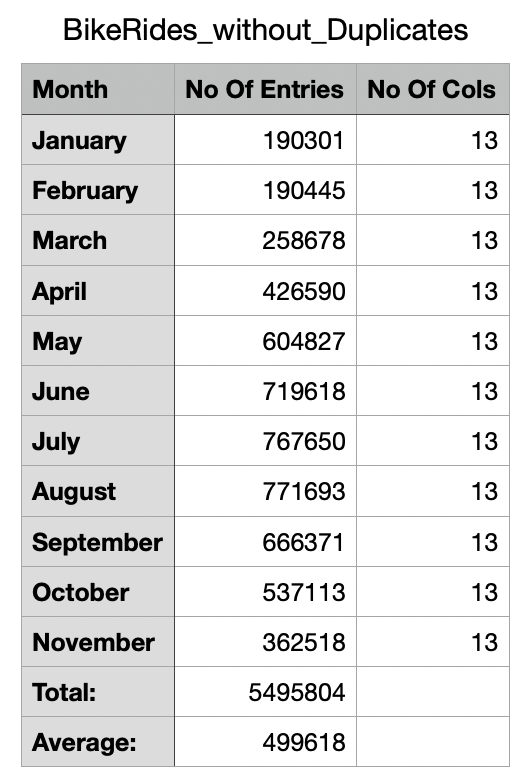
\includegraphics[scale=0.5]{img3.png}
	\end{subfigure}
	\end{figure}
	\pagebreak
	
On the left is the result of running the method without removing duplicates, and on the right is the result after removing duplicates. We can see that all the files have the same number of columns, which is a good preliminary indicator of the consistency of data across the months. In total the dataset contains almost 5.5 Million entries, with an average of approximately 500,000 entries per month. The number of entries before and after removing duplicates is identical, therefore the original dataset did not have any duplicates. \\

	\item \textit{check\_NAN}:\\
	Given that a brief look at the entries from May already showed a couple of NaN values, this method calculates the percentage of NaN values using the pandas function \textit{isna()}. The number of null values for each column is calculated for each month and the results are shown below. As we can see the columns \textit{start\_station\_name}, \textit{start\_station\_id}, \textit{end\_station\_name}, \textit{end\_station\_id} in every month have around 13-17\% null values. The columns \textit{end\_lat} and \textit{end\_long} have less than 1\% null values. 
	\begin{figure}[ht]
	%\hspace{-1.8cm}
	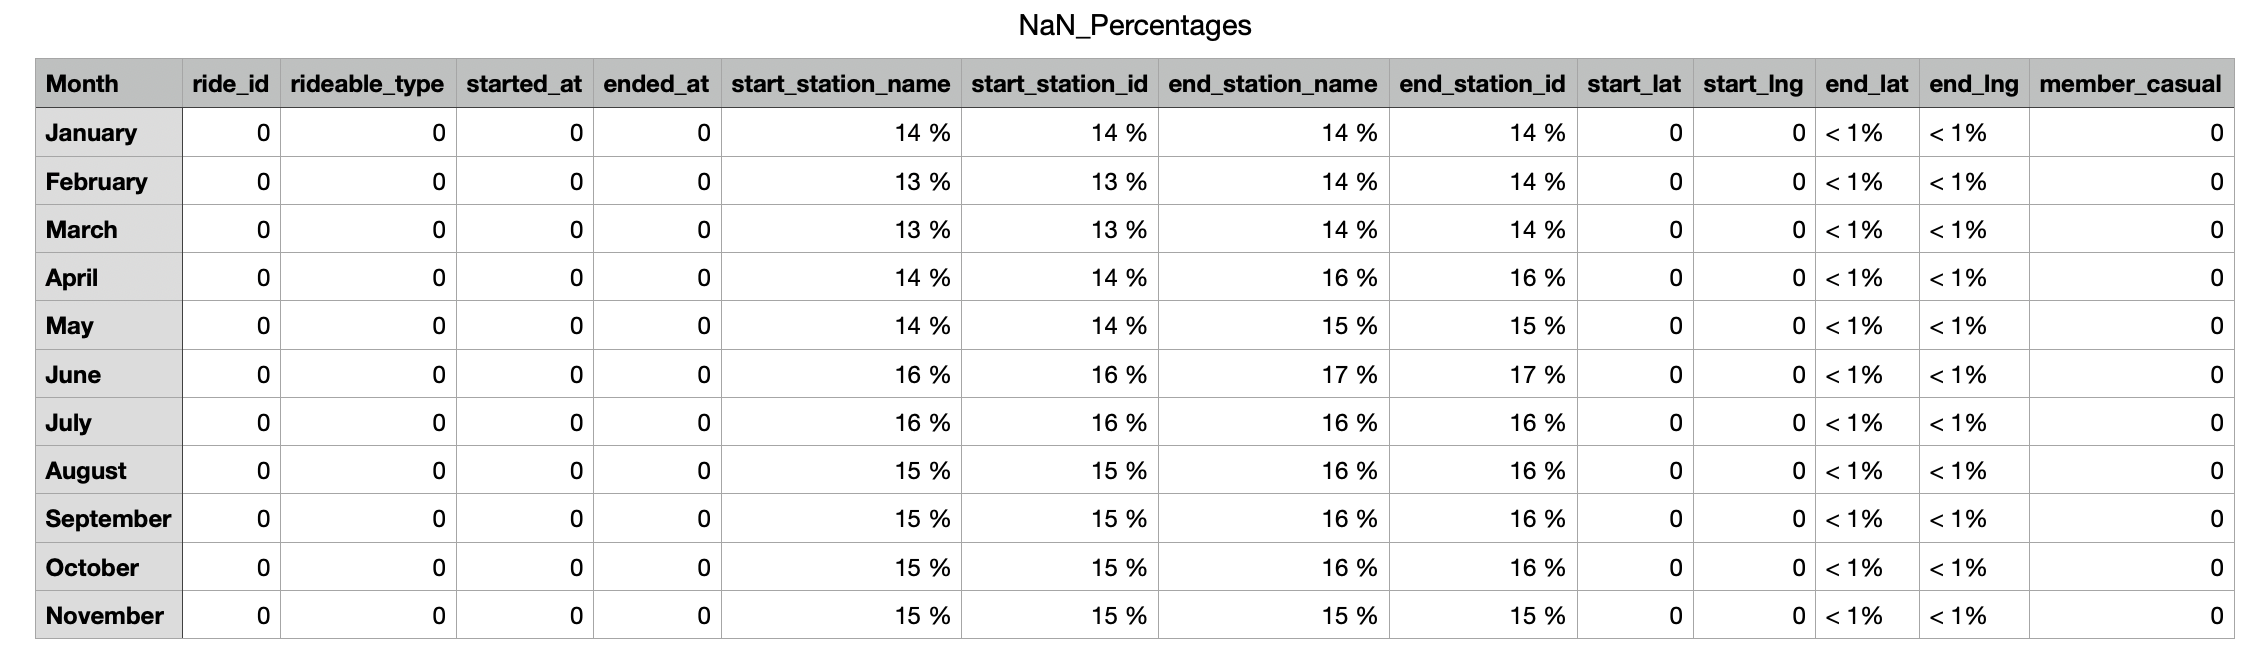
\includegraphics[width=6.5 in, height = 2 in]{imgNAN.png}
	\end{figure}
	
	\item \textit{drop\_NANs}:\\
	Now that the percentage of null values has been identified, the next step is to determine how to deal with these null values. As previously mentioned, the goal of the analysis is to find out how casual riders differ from members. After exploring the dataset, it is clear that this information can be obtained by looking at how the ride lengths vary as well as the type of bikes used. The ride length can be determined either by looking at the time or the distance. Since the information related to the distance contains a lot of null values, it is safer to rely on the time. Therefore, the relevant columns from which this information can be extracted are the: \textit{ride\_id}, \textit{rideable\_type}, \textit{started\_at}, \textit{ended\_at}, \textit{member\_casual}. Which means that we can drop all the other columns which contain the null values. Therefore, the method \textit{drop\_NANs} drops the columns related to start and end stations. After dropping the start and end stations, we can call the method \textit{count\_entries} once again and compare the new dataset shape to the original one:
	
	\begin{figure}[h]
	\centering
	\begin{subfigure}{.4\textwidth}
	\hspace{0.5 in}
		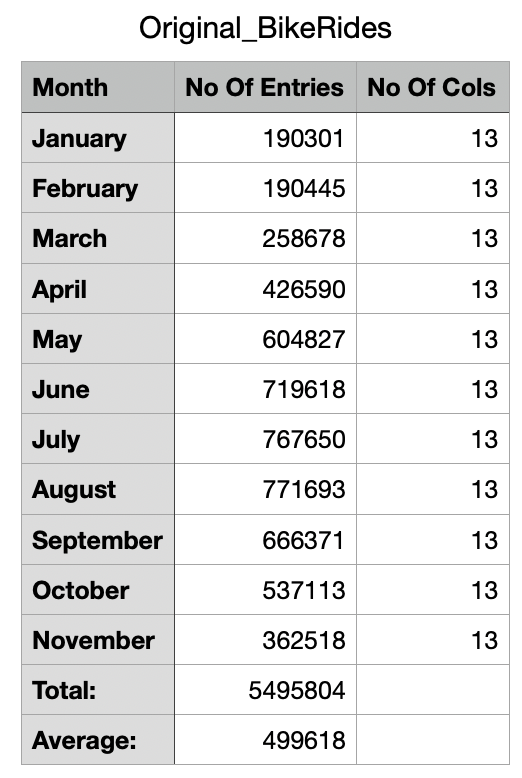
\includegraphics[scale=0.5]{img2.png}
	\end{subfigure}
	\begin{subfigure}{.4\textwidth}
	\hspace{0.5 in}
		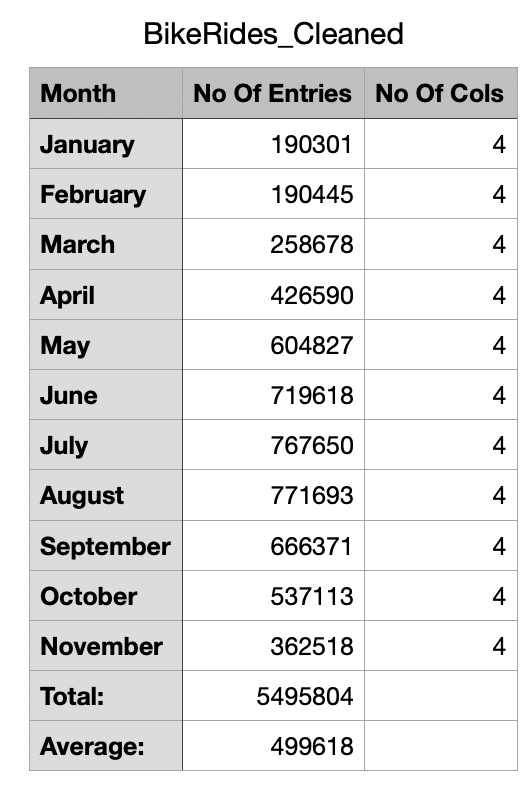
\includegraphics[scale=0.5]{img4.png}
	\end{subfigure}
	\end{figure}
	As expected only the number of columns has changed, and the number of entries remains the same as the original. 
		
\end{itemize} 

\end{document}